% !TEX root = ../main.tex

\chapter{Metodologia}
\label{Chapter3}

La metodologia aplicada en el desenvolupament de NUMEN ha estat un procés híbrid i evolutiu, adaptant-se a les necessitats canviants del projecte i a la corba d'aprenentatge personal. Aquest capítol detalla l'estratègia seguida des de la concepció inicial fins a la implementació final, així com les eines i recursos utilitzats.

\section{Estratègia de Desenvolupament: Dos Temps}

El desenvolupament del projecte s'ha estructurat en dos grans blocs temporals clarament diferenciats, cadascun amb objectius i metodologies pròpies.

\begin{figure}[h]
    \centering
    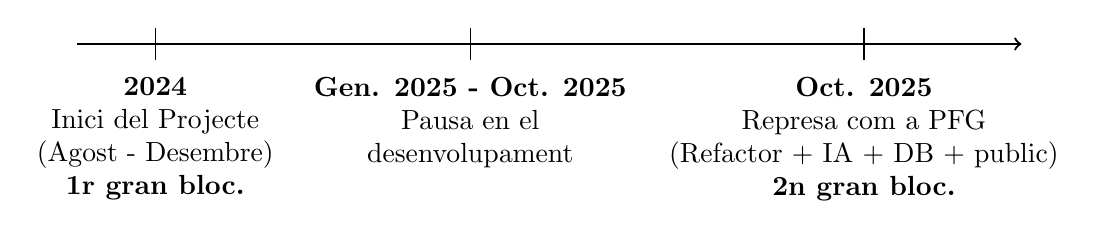
\begin{tikzpicture}
        % Draw the line
        \draw[thick, ->] (0,0) -- (12,0);
        
        % 2022 Node
        \draw (1,0.2) -- (1,-0.2);
        \node[align=center, below] at (1,-0.3) {\textbf{2024} \\ Inici del Projecte \\ (Agost - Desembre) \\ \textbf{1r gran bloc.}};
        
        % 2023 Node
        \draw (5,0.2) -- (5,-0.2);
        \node[align=center, below] at (5,-0.3) {\textbf{Gen. 2025 - Oct. 2025} \\ Pausa en el \\ desenvolupament};

        % Oct 2025 Node
        \draw (10,0.2) -- (10,-0.2);
        \node[align=center, below] at (10,-0.3) {\textbf{Oct. 2025} \\ Represa com a PFG \\ (Refactor + IA + DB + public) \\ \textbf{2n gran bloc.}};
    \end{tikzpicture}
    \caption{Línia temporal del desenvolupament del projecte NUMEN.}
    \label{fig:timeline}
\end{figure}

\subsection{Etapa 1: Naixement i Desenvolupament (2024)}
Aquesta primera etapa, compresa entre l'agost i el desembre de 2024, va néixer d'una forta motivació personal per ajudar a la meva mare, experta en numerologia, a automatitzar els complexos càlculs manuals que requeria la seva feina.

En aquesta primera etapa es van haver de prendre les decisions més importants del projecte, com ara el disseny de l'aplicació, el llenguatge de programació i les tecnologies a utilitzar. El desenvolupament va ser \textbf{purament manual i autodidacta}, sense l'ús d'Intel·ligència Artificial generativa per al codi. Amb l'ajuda de la meva mare i la referència del llibre de Martine Coquatrix, es va assolir la comprensió dels càlculs necessaris per realitzar les cartes numerològiques, ideant algoritmes simples per dur a terme l'automatització d'aquest coneixement.
El resultat d'aquesta fase va ser una aplicació \textbf{completament funcional} a nivell de càlcul: el sistema ja era capaç de generar totes les cartes, mapes i gràfics necessaris. La robustesa del nucli matemàtic de NUMEN és fruit d'aquesta dedicació artesanal, on cada línia de codi va ser escrita i validada manualment, creant una base sòlida i lliure de ``caixes negres''.

Aquest esforç manual atorga un valor afegit al projecte: tot i que avui dia eines com la IA Generativa permetrien aixecar un prototip similar en qüestió de dies, la robustesa i el control absolut sobre la lògica del nucli de NUMEN són totes decisions preses per mi, amb tot el procés evolutiu i reflexiu que comporta, ajudant enormament en el meu procés evolutiu i aprenentatge com a enginyer informàtic.

\subsection{Etapa 2: Professionalització Acadèmica (PFG 2025)}
En reprendre el desenvolupament sota el marc acadèmic del PFG l'octubre de 2025, l'objectiu va virar de la funcionalitat pura cap a la \textbf{professionalització i l'escalabilitat}. En aquest nou context, i conscient de la necessitat real d'adaptar-me a l'evolució tecnològica del sector, aquesta etapa s'ha caracteritzat també per la integració natural d'eines d'Intel·ligència Artificial en el flux de treball diari. 

Lluny de substituir el criteri de l'enginyer, s'ha fet un ús raonable i lògic d'assistents avançats (utilitzant \textbf{Antigravity} com a IDE principal) per accelerar tasques mecàniques, refactoritzar codi i validar hipòtesis tècniques. Aquesta simbiosi home-màquina ha permès abordar reptes complexos amb major agilitat, demostrant que el domini d'aquestes noves eines és ja una competència indispensable per al desenvolupament de programari modern.

Així doncs, en aquesta fase s'han implementat canvis estructurals crítics per convertir una eina d'ús personal en un producte de programari robust:

\begin{itemize}
    \item \textbf{Infraestructura i persistència (Firestore):} Integració de \textbf{Google Firestore} com a base de dades per persistir els estudis. Això ha permès no només guardar les dades, sinó implementar una funcionalitat de \textbf{visualització d'historial} dins la mateixa aplicació, permetent a l'administrador recuperar, consultar i reprendre estudis antics directament des del núvol.
    \item \textbf{Seguretat i autenticació (Login):} Implementació d'un sistema de Login robust amb \textbf{Firebase Authentication} i regles de seguretat (Firestore Security Rules). Aquest pas ha estat imprescindible per protegir la privacitat de les dades davant la nova exposició pública de l'aplicació, assegurant que només l'administrador tingui accés a la informació sensible (noms, dates de naixement).
    \item \textbf{Refactorització de la impressió (Native PDF):} S'ha realitzat un canvi tècnic fonamental en el mòdul d'exportació. A la primera etapa, els informes s'imprimien realitzant una ''captura de pantalla'' del que veia l'usuari, fet que limitava la qualitat. En aquesta etapa, s'ha reescrit el sistema utilitzant llibreries de generació de PDF natiu, codificant plantilles vectorials que repliquen el disseny fidelment però amb qualitat professional, independent de la resolució de la pantalla.
    \item \textbf{Funcionalitat ``Compartir'' i feedback:} S'ha desenvolupat un sistema per generar enllaços temporals segurs (24h) per compartir l'informe amb el client. Aquest sistema inclou ara un mecanisme de feedback bidireccional, on el client convidat pot valorar la precisió de la interpretació mitjançant un sistema de \textbf{puntuació per estrelles (1-5)} i comentaris de text, que queden registrats a la base de dades.
    \item \textbf{Portal públic i divulgació:} Creació d'una nova àrea pública (\textit{Landing Page}) per captar l'interès de nous usuaris. Aquesta secció inclou contingut teòric educatiu (House Tour, conceptes bàsics), una ``Demo'' interactiva que permet calcular el Camí de Vida de manera gratuïta, un mur de \textbf{Testimonis} (Social Proof) i un accés directe a \textbf{WhatsApp} per contractar serveis professionals.
    \item \textbf{Disseny responsive:} Refactorització de la interfície per garantir la usabilitat en dispositius mòbils i tauletes, adaptant els gràfics complexos a pantalles petites.
    \item \textbf{Integració d'IA (Gemini):} Finalment, s'ha connectat l'API de Gemini (model Flash) per a la interpretació de les dades i la generació dels informes. És important notar que la IA només s'utilitza per enriquir el resultat amb text natural; no intervé en els càlculs, mantenint la fiabilitat de l'etapa anterior.
\end{itemize}

\section{Metodologia de Treball}
S'ha seguit una adaptació personalitzada de les metodologies àgils, prioritzant l'entrega contínua de valor mitjançant cicles iteratius que permeten una adaptació flexible als canvis. Donat que l'equip està format per una única persona, en lloc de \textit{Sprints} rígids tipus Scrum, s'ha optat per un enfocament incremental:
\begin{enumerate}
    \item \textbf{Disseny Inicial:} Definició de l'arquitectura i model de dades.
    \item \textbf{Implementació per Prioritats:} Codificació dels mòduls més influents i crítics (motor de càlcul) abans d'abordar la interfície d'usuari o la generació d'informes.
    \item \textbf{Refactorització Contínua:} Revisió constant del codi per millorar-ne l'eficiència i la llegibilitat a mesura que s'adquirien nous coneixements.
\end{enumerate}

\section{Declaració d'Ús d'Intel·ligència Artificial}
D'acord amb la normativa acadèmica i els principis de transparència, es declara explícitament l'ús d'eines d'Intel·ligència Artificial Generativa en aquest Treball Final de Grau.

\begin{itemize}
    \item \textbf{Desenvolupament de Software:} El nucli de l'aplicació, l'arquitectura i la lògica de negoci han estat desenvolupats manualment des de l'any 2024. L'ús d'IA en el codi s'ha limitat recentment a tasques de suport puntual, com la generació de consultes complexes a la base de dades o l'optimització de funcions específiques de \textit{prompting}.
    \item \textbf{Redacció de la Memòria:} S'han utilitzat models de llenguatge (com Google Gemini) com a assistents de redacció per a la revisió d'estil, correcció ortogràfica i estructuració de continguts, amb l'objectiu d'assolir un nivell de professionalitat i formalitat acadèmica excel·lent.
    \item \textbf{Autoria:} Tot el contingut generat o suggerit per la IA ha estat revisat, validat i editat exhaustivament, mantenint la responsabilitat total sobre la veracitat i originalitat del treball presentat. La IA ha servit com a eina d'amplificació de capacitats, no com a substitut de l'autoria intel·lectual.
\end{itemize}
